\documentclass[a4paper,12pt]{article}
\usepackage{indentfirst,latexsym,bm}
\usepackage{indentfirst}
\usepackage[natural]{xcolor}
\usepackage{amsmath}
\usepackage{indentfirst}
\usepackage{ctex}
\usepackage{geometry}
\usepackage{indentfirst}
\usepackage{setspace}
\usepackage{graphics}
\usepackage{diagbox}
\usepackage{array}
\usepackage{booktabs}
\usepackage{graphicx}
\usepackage{float}
\usepackage{amssymb}
\newcommand{\song}{\CJKfamily{song}}    
\newcommand{\fs}{\CJKfamily{fs}}     
\newcommand{\kai}{\CJKfamily{kai}}   
\newcommand{\hei}{\CJKfamily{hei}}     
\newcommand{\li}{\CJKfamily{li}}       
\newcommand{\you}{\CJKfamily{you}}    
\newcommand{\chuhao}{\fontsize{42pt}{\baselineskip}\selectfont}     
\newcommand{\xiaochuhao}{\fontsize{36pt}{\baselineskip}\selectfont} 
\newcommand{\yichu}{\fontsize{32pt}{\baselineskip}\selectfont}      
\newcommand{\yihao}{\fontsize{28pt}{\baselineskip}\selectfont}     
\newcommand{\erhao}{\fontsize{21pt}{\baselineskip}\selectfont}      
\newcommand{\xiaoerhao}{\fontsize{18pt}{\baselineskip}\selectfont}  
\newcommand{\sanhao}{\fontsize{15.75pt}{\baselineskip}\selectfont}  
\newcommand{\sihao}{\fontsize{14pt}{\baselineskip}\selectfont}      
\newcommand{\xiaosihao}{\fontsize{12pt}{\baselineskip}\selectfont}  
\newcommand{\wuhao}{\fontsize{10.5pt}{\baselineskip}\selectfont}    
\newcommand{\xiaowuhao}{\fontsize{9pt}{\baselineskip}\selectfont}   
\newcommand{\liuhao}{\fontsize{7.875pt}{\baselineskip}\selectfont}  
\newcommand{\qihao}{\fontsize{5.25pt}{\baselineskip}\selectfont}    
\newcommand{\gx}{G^{\times}}
\begin{document}
	\begin{spacing}{1.2}
		\wuhao
		\section{第一题}
		\subsection{网络的建立}
		利用题目所给出的influence数据集可以建立以artist为节点的有向网络,规定网络的方向是由follower指向influencer,即对于相连接的两个节点对于follower而言是出边,对于influencer而言入边.并可以给出邻阶矩阵$\bm{A}$为$A_{ij}$.
		\subsection{参数建立}
		为了获取能够表征artist(节点)影响力的参数,我们希望借助网络已经有的常用参数(特征路径长度,聚合系数,度中心性)来描述.下面先列出各个参数,再逐个分析其在该问题表示的实际意义.
		\subsubsection{特征路径长度(characteristic path length)}
		在无向图中可以定义特征路径长度,在无向图中网络的特征路径长度指网络中所有节点对的平均路径长度,两点之间的路径长度$L_{ij}$为连接两点的最短路径上所包含的边的数目.
		\par
		而在我们讨论的问题中需要做出相应修改,首先将特征路径的概念限制在结点i.依据其为有向图的特点,只考虑i结点入边所连接的点,这些点的连接点同理也只考虑由出边所连接的部分,已经讨论过的点不再加入(避免出现同一层相连的情况).利用前述的点可以定义出以结点i为根节点的树(不考虑环的情况)记为$T(i)$,因此子图每一个节点的入度也就是子树数目.每一个节点j到节点i的路径长度$L_{ij}$即为节点j的深度.如果将子图$T(i)$中每一片叶子节点(入度为0的点)的深度相加再除以i的入度,就可以描述平均一个i的子树的深度,定义此量可以用来描述结点i影响的深度.为了方便描述,引入子图$T(i)$对应树的叶结点的集合$T_{l}(i)$.结点i对应的特征路径长度$L(i)$为,结点i的入度为$k_{i}$
		$$
		L(i)=\sum\limits_{j\in T_{l}(i)}\frac{L_{ij}}{k_{i}}
		$$
		该参数越大表示artist的影响力越深远.
		\subsubsection{聚合系数(clustering coefficient)}
		假设某个节点有k条边(出边和入边之和),则这k条边连接的节点((k个)之间最多可能存在的边的条数为$\frac{k(k−1)}{2}$,用实际存在的边数除以最多可能存在的边数得到的分数值,定义为这个节点的聚合系数.反映了同一影响者的追随者之间,也存在影响关系的程度,聚合系数是网络的局部特征.聚类系数越大,表示该点也越容易参与组成一个多元结构,表明此类影响有更强的凝聚性产生一系列的影响.记与i相邻的点的集合为B(i).
		$$C(i)=\frac{2}{k(k-1)}\sum\limits_{j,k\in B(i)}(A_{kj}+A_{jk})$$
		\subsubsection{katz中心性}
		在此参数在图中虽然都能体现影响力,但是都属于局部性质,涵盖的信息有限,为了更加全面的反映影响力,下面引入katz的中心性的概念.
		\par
		The Katz influence matrix $I_{k}$ is defined via
		$$
		\bm{I_{K}}=(\bm{I}-\alpha \bm{A})^{-1}-\bm{I}
		$$
		where $\bm{I}$ is an identity matrix, $\bm{A}$ is the adjacency matrix as before, and $\alpha$ is a decay factor which scales the indirect influence allowed to propagate though the network(larger $\alpha$ imp;oes greater weight on indirect influence). This can be written in equivalent from as
		$$
		\bm{I}_{K}=\alpha\bm{A}+{\alpha}^{2}\bm{A}^{2}+\cdots+{\alpha}^{k}\bm{A}^{k}+\cdots
		$$
		where we can see that the influence is a weighted sum of the powers of the adjacency matrix. When the values of $\bm{A}$ are zero or one, the powers of the adjacency matrix $\bm{A}^k$ have elements representing the number of sample chains of corresponding length k capturing various levels of indirect influence.For stability,
		$\frac{1}{\alpha}$ must be greater than the largest eigenvalue of A and for large networks.
		\par
		 Given $\bm{I}_{K}$, we can view the column of a node to find who influenced the node, or view the row of the node to find who the node influenced. Summing the columns of the influence matrix produces a ranking of the most influential nodes, while summing the rows results in a ranking of the most influenced nodes.
		 \par
		 有了上面三个参数特:\textbf{征路径长度L(i)},\textbf{聚类系数C(i)},\textbf{katz中心性}$\bm{I_{K}}$就可以建立起衡量音乐影响力的标准,进而作为 the parameters that capture ‘music influence’.
		 \subsection{Creating a subnetwork of directed influencer network} 
		 下面对前述建立的网络进行划分,由于网络本身具有社区结构特性,所以通过社区检测(community detection)技术可以对网络的节点进行据类.下面将主要采用Newman的最佳模块化方法(The Method of Optimal Modularity).引入模块化参数Q来描述网络划分的好坏程度.其中Q的定义如下
		 $$
		 Q=\frac{1}{4m}\sum\limits_{ij}\left(A_{ij}-\frac{k_{i}k_{j}}{2m}\right)(s_{i}s_{j}+1)=\frac{1}{4m}\sum\limits_{ij}\left(A_{ij}-\frac{k_{i}k_{j}}{2m}\right)s_{i}s_{j}
		 $$
		 其中$k_{i}$表示结点i的度(出度和入度之和),$m=\frac{1}{2}\sum\limits_{i}k_{i}=\frac{1}{2}\sum\limits_{ij}A_{ij}$上面对Q的定义基于将一个集合分类为2个,因此s的意义为,当i属于其中一个元素取+1,另一个则取-1.所以问题转化为求取一个$\bm{s}$使得Q的值最大.(注意Q可为正也可为负.Q越大表示分割的社区越合理,为0表示没有进行分割).对Q的表达式进行化简
		 $$
		 Q=\frac{1}{4m}\bm{s^{T}}\bm{B}\bm{s}=\frac{1}{4m}\sum\limits^{n}_{i=1}(\bm{u_{i}^{T}}\bm{s})^{2}\beta_{i}
		 $$
		 其中$B_{ij}=A_{ij}-\frac{k_{i}k_{j}}{2m}$而$\beta$是$\bm{B}$的特征值,$\bm_{i}$为其正交归一化的特征向量,如果$\beta_{1}\geqslant\beta_{2}\geqslant\cdots\geqslant\beta_{n}$.我们希望通过选择适当的网络划分或等效地通过选择向量$\bm{s}$的值来最大化模块化Q.由于Q涉及最大(正)特征值.我们希望$\beta_{1}$的系数较大,即$(\bm{u_{i}^{T}}\bm{s})^{2}$越大,也就是$\u_{1}$与$\bm{s}$尽可能靠近,所以将$\bm{s}$的符号取得同$\bm{u}_{1}$一致即可,同时因为$\bm{s}$与$\u_{1}$接近由于实对称矩阵的特征向量正交使得其他特征值对应的系数较小.
		 \par
		 前面完成了分为两个社区的工作,下面需要将分开的两个社区进一步划分,但是考虑到全局的最优化问题需要将相应的模块化参数Q进行修改
		 $$
		 \Delta Q=\frac{1}{2m}\left[\frac{1}{2}\sum\limits_{i,j\in g} B_{ij}(s_{i}s{j}+1)-\sum\limits_{i,j\in g}B_{ij}\right]=\frac{1}{4m}\bm{s^{T}}\bm{B^{(g)}}\bm{s}
		 $$
		 其中g为上述分割过的其中一个集合,$B_{ij}^{(g)}=B_{ij}-\delta_{ij}\sum\limits_{k\in g}B_{ik}$,利用前述方法进行分割求得$\bm{s}$即可.
		 \par
		 利用igraph中的函数community\_fastgreedy,可以实现上述的算法.在$\bm{B}^{(g)}$没有正的特征值时可以停止分割,同时也可人为设定分割次数.对此问题如果以上标准分为29块,但是为了更好的分析问题忽略次要因素,我们人为的将模块数定为16块.计算得到Q=0.454.
		 \subsection{结果分析}
		 可以看出社区的数量明显少于流派的数量.这说明了流派之间存在相互影响,这个问题将会在后面讨论.这里仅仅讨论一个社区内的结构.对社区内的结点求在该社区内的征路径长度$L^{(g)}(i)$,聚类系数$C^{(g)}(i)$,katz中心性$\bm{I}^{(g)}_{K}$可以发现在社区内具有音乐影响力的个别结点.这符合网络的\textbf{无标度特性}.即便是在子途中我们也可以发现每一个社区都存在一些影响力极大,或是影响力深渊的artist.他们对整个社区的形成有贡献.下面来阐述每一个参数在某1个社区中的含义.\\
		 \textbf{特征路径长度}:可以找到特征路径长度最大的节点,其有可能就是该社区中最有音乐影响力的artis.从影响力的深度而言可以用参数衡量.\\
		 \textbf{聚类系数}:此参数在社区中是衡量社区的紧密程度的,单个节点的聚类系数也可以说明社区中个别点的影响力强度.用以衡量影响力强度可以此参数衡量.如下图所示,左侧的社区显然比右侧的社区更加紧密,右侧更加发散.说明左边的社区中很可能存在聚类系数很大的节点,且其影响力极强.
		 \begin{figure}[!ht]
		 	\begin{center}
		 		\begin{minipage}{0.47\linewidth}
		 			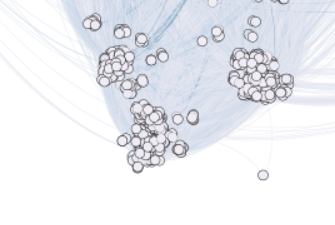
\includegraphics[scale=0.5]{c1.png}
		 			\caption{紧密型社区}
		 		\end{minipage}
		 		\begin{minipage}{0.45\linewidth}
		 			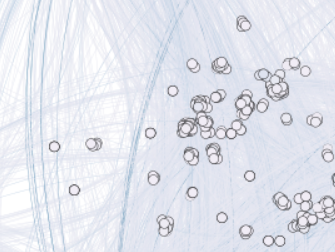
\includegraphics[scale=0.47]{c2.png}
		 			\caption{发散型社区}
		 		\end{minipage}
		 	\end{center}
		 \end{figure}\\
	 \textbf{katz中心性}:此参数在影响力排名和综合影响力(深度与强度)上有更强的代表性.在一个子网络中求出对应的中心性$\bm{I}^{(g)}_{K}$按照前述的做法,将$\bm{I}^{(g)}_{K}$的列相加得到最具有影响力的点.这时考察这些点所属的流派可以将社区归属于某个社区.然后统计最具影响的节点所属流派在此社区的占比.(平均占比在80\%左右),所以大部分情况可以用最具有影响力的节点所属流派标注某个社区.
	\section{第二题} 
	为了刻画音乐的相似程度我们需要在首曲子之间建立一种距离,需注意的是,通常我们是基于某种形式的距离来定义"相似度度量",距离越大,相似度越小.但是用于相似度度量的距离未必定要满足距离度的所有基本性质(正定性,对称性,直递性),尤其是直递性(三角不等式).此时该距离不再满足直递性;这样的距离称为"非度量距离".这时我们引入的距离就是一种非度量距离.
	\subsection{数据处理}
	\par 不同音乐之间距离的建立依托于其音乐特征,用向量$\bm{x}$来表示,在定义距离之前需要对数据进行处理.数据的维数过大带来处理不便,同时有些参数对距离的贡献不大因此可以略去.通过观察除了explicit和mode是0.1取值外,其余各量均为连续取值,而explicit中有96\%以上的取值为0所以此因素不予考虑.剩下13个量我们将用主成分分析的方法进行聚合减少变量的个数,记某个音乐特征为$y_{i}\quad (i=1\cdots13$).
	\subsubsection{数据标准化}
	剩余的13个变量各个范围不同,这造成了标准的不一致,使得主成分分析有较大的误差,对数据进行下面的标准化
	$$
		Z_{i}(y_{i})=\frac{y_{i}-\overline{y}_{i}}{S(y_{i})}=\frac{y_{i}-\overline{y}_{i}}{\sqrt{\frac{(y_{i}-\overline{y}_{i})^{2}}{{n-1}}}}
	$$
	\subsubsection{主成分分析}
	在对数据进行标准化后进行主成分分析,成分分析法是一种降维的统计方法,它借助于一个正交变换,将其分量相关的原随机向量转化成其分量不相关的新随机向量,这在代数上表现为将原随机向量的协方差阵变换成对角形阵,在几何上表现为将原坐标系变换成新的正交坐标系,使之指向样本点散布最开的几个正交方向,然后对多维变量系统进行降维处理,使之能以一个较高的精度转换成低维变量系统.
	在这个问题中我们使用主成分分析的方法得到聚合后的变换矩阵,而转化后的数据我们仅需要取前几项(贡献率大的几项),这里我们取4项目,为了方便叙述,降维后的音乐特征参数还是选用$\bm{x}$来描述.
	\par
	从主成分分析的变换矩阵中我们可以观察出某些相关的影响因素,下面就以其中贡献度最大的4个变量构成情况来分析.完整表格见附件.
\begin{table}[H]
		\centering
		\setlength{\tabcolsep}{2.0mm}{
			\caption{贡献最大的4个变量的构成}
			\begin{tabular}{ccccc}
				\toprule[1.2pt]
				&相关变量1&相关变量2&相关变量3&相关变量4\\
				\hline
				$x_{1}$&energy(0.48)&loudness(0.47)&danceability(0.22)&popularity(0.32)\\
				$x_{2}$&danceability(0.56)&valence(0.51)&acousticness(0.20)&duration(-0.0.42)\\
				$x_{3}$&liveness(0.62)&acousticness(0.60)&speechine(0.13)&popularity(-0.15)\\
				$x_{4}$&mode(0.67)&tempo(0.23)&key(-0.52)&loudness(0.66)\\
				\bottomrule[1.5pt]
		\end{tabular}}
\end{table}
从上述可以看出经过主成分分析后的参数数量减少,每一个参数是由多个参数聚合而成蕴含了更多的信息,比如从上面的表格可以看出$x_{1}$表征的是冲击感,响度的参数即energy和loundness总是有一定的关联性.有如$x_{3}$其中liveness和acousticness占有大比例,说明此参数能够刻画作品给人的现场感和对合成电音或是纯音乐的运用程度.但是并非所有的主成分分析的参数都能够有明确的实际意义,但是在后面定义相似度的距离中已经足够了.
\subsection{定义距离}
\subsubsection{任意两作品之间的距离}
对于任意两个作品i,j都有对应的参数$\bm{x}$,将所有作品或者(artist)看作一个具有音乐特征的元素(点),分布在音乐特征空间(space)中,定义两个作品的距离为
	$$
	d(x(i),x(j))=\sqrt{\sum\limits_{n=1}^{4}\left( x_{n}(i)- x_{n}(j)\right)^{2}}
	$$
	有了距离就可以描述两个作品的相似程度.距离越近越相似,越远差异越大.类似的,不同artist的距离可以通过求出其作品的均值后再运用上面的公式计算\\
	\subsubsection{流派半径}
	对于某个流派的作品的相似程度我们用下面的方法描述,定义流派的半径:
	$$
	r=\frac{1}{N}\sum\limits_{i=1}^{N}d(x(i),\overline{x})=\overline{d(x(i),\overline{x})}
	$$
	其中N为某个流派的artist的数量,x(i)为第i个artist的音乐特征,$\overline{x}=\frac{1}{N}\sum
	\limits_{i=1}^{N} x(i)$为音乐特征的均值,将此点取为球心.r即为N个artist到均值点距离的均值.示意图如下.
	\begin{figure}[!h]
		\begin{center}
			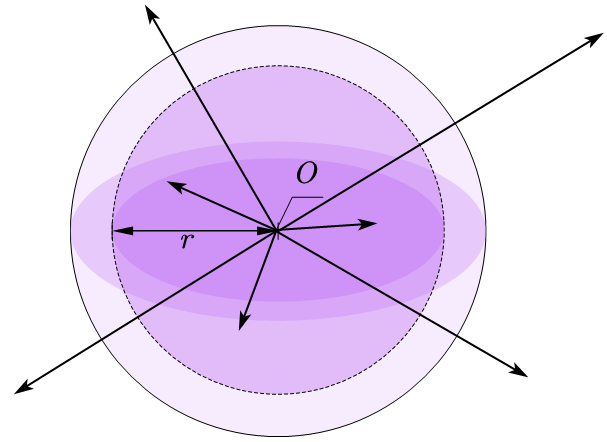
\includegraphics[scale=0.45]{dis1.png}
			\caption{同一流派的类似程度}
		\end{center}
	\end{figure}
通过比较流派半径可以知道是否该流派作曲家的作品更加相似,在音乐特征空间更为接近.
\subsection{结果分析}
下面来回答问题,是否同一流派的音乐家创作的作品更加相似.首先通过influence\_data文件找到artist和其所属流派的关系,将此关系应用于data\_by\_artist文件,标注流派信息.按照流派分类后,执行上述算法.观察发现,给出的artist的信息分布不均匀,如Pop/Rock和R\&B,reggae占了大部分.下面举例将只提及部分.其余见附件.
\begin{table}[H]
	\centering
	\setlength{\tabcolsep}{3mm}{
		\caption{几个流派半径的比较}
		\begin{tabular}{cccccc}
			\toprule[1.5pt]
			random&Pop/Rock&R\&B&reggae&Folk&Classical\\
			\hline
			24.02&1.84&1.75&1.69&1.51&1.52\\
			\bottomrule[1.5pt]
	\end{tabular}}
\end{table}
其中random是在所有artist中随机抽取1000个样本,再按照前述的计算方法得到的结果.相当于假设作品的相似程度和所属流派无关.可以发现如果假设成立,则不应该出现random的流派半径和取定流派计算得到的流派半径差距如此悬殊.因而说明同一流派的artist之间的作品更加相似.同时也能发现流派的数据越多,或者我们猜测从事此流派的artist人数越多,其半径越大,表示此流派越开放子种类越多,范围越广.
\section{第三题}
前面定义了不同作品和不同artist之间的距离,其本质都是音乐特征空间中元素的距离,流派半径可以理解为音乐特征空间中的子集的性质.在这个问题中我们要讨论流派之间的关系(异同,以及相互之间的影响),所以我们要定义出流派之间的关系下面我们定义不同流派之间的距离和亲和度.
\subsection{流派距离}
首先我们知道两个流派是有各自的流派半径r的,这时候我们可以考虑利用流派半径来构造流派之间的距离,假设两个流派的流派半径分别是$r_{i}$和$r_{j}$,其球心的坐标分别为$\overline{x}_{i}$和$\overline{x}_{j}$定义流派距离
$$
\widetilde{d}(i,j)=d(\overline{x}_{i},\overline{x}_{j})-r_{i}-r_{j}
$$
注意$\widetilde{d}$和d是不同意义的距离,前者是流派与流派之间,后者是artist与artist之间$d(\overline{x}_{i},\overline{x}_{j})$表示的是流派中心点(artist的均值)之间的距离.这里没有考虑距离变为负值的情形,从前述可以看出不同流派中心的距离是很大的可以认为$d(\overline{x}_{i},\overline{x}_{j})\geqslant r_{i}-r_{j}$总是成立的.示意图如下:
	\begin{figure}[!h]
	\begin{center}
		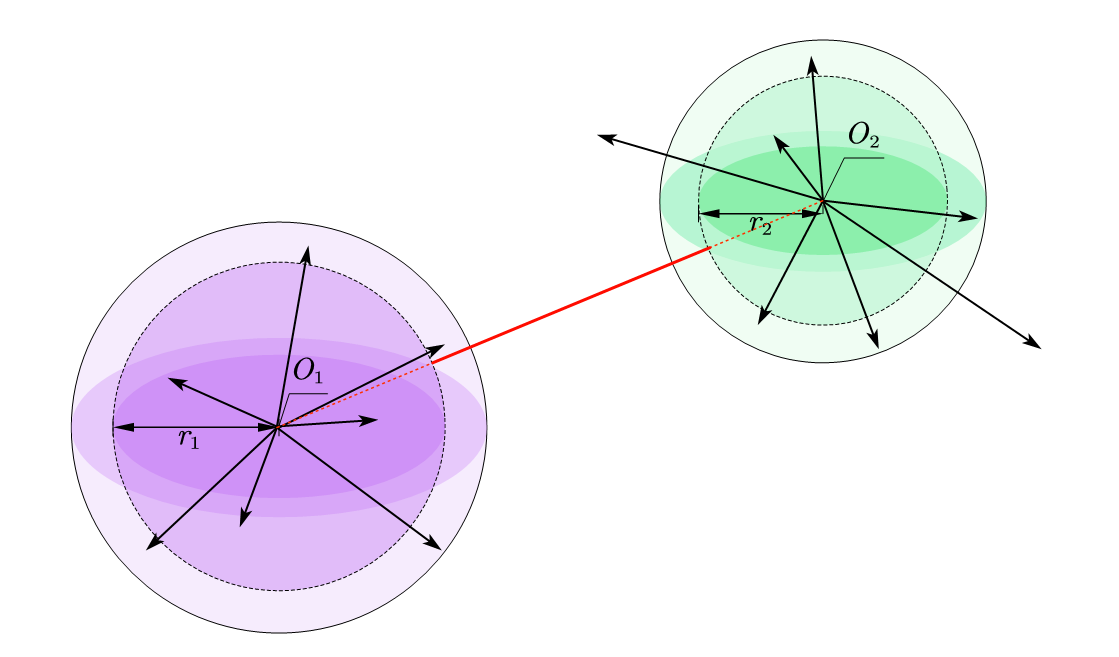
\includegraphics[scale=0.25]{dis2.png}
		\caption{流派距离示意图}
	\end{center}
\end{figure}\\
类似前面所述的关于artist和作品的距离,利用流派距离的概念可以在一定程度上可以描述两个流派的差异.下面利用流派距离寻找两个流派之间的相似点和差异.
\subsection{相似与差异}
如示意图所示,红色实线的长度在一定程度上上能够反映差异的程度,而我们希望能够找到哪些音乐特征存在具体的差异.设向量$\Delta\bm{x}=\overline{\bm{x}}_{i}-\overline{\bm{x}}_{j}$.我们可以通过考察$\Delta\bm{x}$的分量来寻找两个流派之间的差异.经过主成分分析后的4个聚合量我们只要找到那个量差异最大,其指标为M,哪个量差异最小,其指标为m.(m与M都在1-4取值).
$$
|\Delta x_{M}|=\max\limits_{1\leqslant n\leqslant4}|\Delta x_{n}|\qquad |\Delta x_{m}|=\min\limits_{1\leqslant n\leqslant4}|\Delta x_{n}|
$$
其中$\Delta x_{n}$表示$\Delta\bm{x}$的分量.在找到对应的$x_{M}$和$x_{m}$后,我们利用PCA中得到的正交变换矩阵寻找两个流派之间最相似和差异最大的分量.(没有PCA的变量记为$\bm{\gamma}$)从前面可知有$\bm{x}_{4 \times 1}=\bm{R}_{4\times 13}\bm{\gamma}_{13\times 1}$,其中系数矩阵$\bm{R}$由附件给出.找到M和m后就可以将系数矩阵中$R_{Mi}$和$R_{mi}$提取出来排序,其中$|R_{Mi}|$越大的对应的$\gamma_{i}$是差异较大音乐特征,反之$|R_{mi}|$越大的对应的$\gamma_{i}$是差异较小音乐特征.
\par
上面只是比较了两个流派之间的差异,如果想衡量差异的程度可以考虑结合流派距离.如前所属如果我们找到了对应于最大差异因素和最小差异的指标M和m,那么可以流派距离在这两个方向上的投影.且由于PCA变换后的坐标具有正交归一性.写成向量形式为
$$
\widetilde{d}(i,j)_{M}=\widetilde{d}(i,j)\frac{\Delta\bm{x}^{T}\cdot\bm{\xi}^{M}}{(\Delta\bm{x}^{T}\Delta\bm{x})^{\frac{1}{2}}}\qquad
\widetilde{d}(i,j)_{m}=\widetilde{d}(i,j)\frac{\Delta\bm{x}^{T}\cdot\bm{\xi}^{m}}{(\Delta\bm{x}^{T}\Delta\bm{x})^{\frac{1}{2}}}
$$
其中$\bm{\xi}^{m}$是对应的第m个变量方向的单位向量.上面两个量可以定量分析差异和相似的程度.
\subsection{相互影响的评定}
下面建立描述流派之间相互影响的参数.流派亲和度
\vspace{15cm}
 \begin{table}[H]
 	\centering
 	\setlength{\tabcolsep}{1mm}{
 		\caption{各个流派的半径的方差}
 		\begin{tabular}{ccccccccccc}
 			\toprule[1.5pt]
 			genre&Pop/Rock&Latin&Jazz&R\&B&International&Country&Classical&Electronic&Stage\&Screen&Comedy\_Spoken\\
 			\hline
 			mean&1.84&1.63&1.82&1.75&1.83&1.45&1.52&2.00&1.65&1.70\\
 			var&0.64&0.41&0.61&0.49&0.68&0.42&0.58&0.71&0.68&1.19\\
 			\bottomrule[1.5pt]
 	\end{tabular}}
  \begin{tabular}{ccccccccccc}
 	\toprule[1.5pt]
 	genre&Easy Listening&Vocal&Reggae&Blues&New Age&Religious&Folk&Unknown&Avant-Garde&Children's\\
 	\hline
 	mean&1.18&1.74&1.69&1.53&1.09&1.71&1.50&0.25&1.08&1.12\\
    var&0.29&0.54&0.46&0.33&0.34&0.34&0.57&0.03&0.21&0.22\\
 	\bottomrule[1.5pt]
\end{tabular}
 \end{table}	
\end{spacing}
\end{document}